\documentclass[9pt, twocolumn]{article}
\usepackage{amsmath, indentfirst, epsfig, ifthen, booktabs, multirow}
\usepackage{nomencl}
\makenomenclature

\renewcommand{\nomgroup}[1]{%
%\ifthenelse{\equal{#1}{A}}{\item[\textbf{Roman Symbols}]}{%
\ifthenelse{\equal{#1}{G}}{\item[\textbf{Greek Symbols}]}{%
\ifthenelse{\equal{#1}{C}}{\item[\textbf{Abbreviations}]}{%
\ifthenelse{\equal{#1}{S}}{\item[\textbf{Subscripts}]}% matches mathematical symbols
}% matches Subscripts
}% matches Abbreviations
}% matches Greek Symbols
}% matches Roman Symbols

\makeindex
\begin{document}

\title{Cascade system using both trough system and dish system for power generation}
\date{}
%\author{Cheng Zhang}
\maketitle


\newpage{}

\section{Introduction}
%\begin{itemize}
%    \item Background Information
%    \begin{enumerate}
%        \item Why do we need cascade system
%        \item What is the advantage of cascade system
%        \item What are others' works
%        \item What have been done
%        \item What to be done
%        \item What can we improve
%        \item What have we done
%    \end{enumerate}
%    \item System specification
%    \begin{enumerate}
%    	\item Environment
%	\item Trough collector
%	\item Dish collector
%	\item Steam turbine
%	\item Stirling engine
%    \end{enumerate}
%    \begin{enumerate}
%    	\item Air circuit
%	\item Water circuit
%	\item Oil circuit
%	\item System efficiency
%    \end{enumerate}    
%    \item Separate system
%    \item Results
%\end{itemize}

Energy is the crucial part for the infrastructure and maintenance of  society. With the increase amount of energy consumption, our quality of life has been improved significantly. However, nowadays the world energy consumption is highly dependent on fossil fuels, which supplied 81.3\% of the world's energy consumption in 2012 according to the data of World Bank Group. Using fossil fuels a lot is afflicting the environment, which is sacrificing our quality of life. Environmental pollutions and global warming are becoming serious problem, and it is urgent to find clean and renewable energy to substitute the fossil fuels.

Solar energy is a clean, sustainable, wide-distributed energy. The total amount of solar energy is very huge. The amount of sunlight striking the earth's atmosphere continuously is 1.75$\times10^{5}\,$TW, even if 1\% of it could be converted into electric energy with a 10\% efficiency, it would produce 175 TW, much larger than the total global energy needs predicted to be 25?30 TW in 2050\cite{goswami2015}. But at the same time, solar energy has some disadvantages for its low flux density and large fluctuation due to daily and seasonal variations exacerbated by variations owing to weather. Concentrated solar power (CSP) technology has the ability to overcome these disadvantages and believed to be the future power generation technology.

There are 4 common forms of CSP technologies, parabolic trough, dish Stirlings, concentrating linear Fresnel receiver, and solar power tower. Different types of collectors and different technologies for electricity generation are suitable for different working temperature zones with different costs. Combination of different collectors with different technologies may provide a new direction to achieve higher efficiency with lower cost for CSP.

Cau\cite{Cau2014} reported a comparative performance analysis of CSP plants using parabolic trough and linear Fresnel collectors, thermal oil as heat transfer fluid and an Organic Rankine Cycle (ORC) power generation unit. A two-tank direct thermal storage system are included and in the Rankine cycle, regenerator, 4~6 steam extractions and air-cooler condenser are used. The performance analysis of the two types of system shows that CSP plants based on linear Fresnel collectors lead to higher values of electrical energy production per unit area of land and CSP plants based on parabolic troughs gives better values of energy production per unit area of collector.

Franchini\cite{Franchini2013} carried out simulations to predict the performance of a Solar Rankine Cycle (SRC) and an Integrated Solar Combined Cycle (ISCC) when combined with two different solar field configurations based on parabolic trough collectors (PTCs) and power tower (PT) systems. The comparative analysis was mainly focused on the influence of CSP technology on global solar energy conversion efficiency of both SRC and ISCC plants. Results show that both higher collection efficiency and conversion efficiency of ST compared to PTCs in both SRC and ISCC situations.

Cipollone\cite{Cipollone2014} discussed some thermodynamic and engineering aspects concerning the use of parabolic troughs for heating gasses of gas turbines. They further discussed the Discrete Ericsson Cycle (DEC), in the cycle, a sequence of intercooled compressions and reheated expansions is deployed to increase cycle specific work and efficiency. They applied optimization adopting as design parameter the power per unit of collector length, and pointed out that the number of compressions and expansions could not exceed three stages.

Behar\cite{Behar2014} reviewed the R\&D activities and published studies on integrated solar combined cycle system (ISCCS), various configurations have been proposed with their performance investigated. The paper also introduced lots of software or mathematical programs to simulate the performance of various design.

Ghaem\cite{Ghaem2012} investigated and compared the performance of various configurations of hybrid solar dish-Brayton cycle. A thermodynamic model implemented in Engineering Equation Solver (EES) is developed for various configurations. Results show that the model in which receiver located before the turbine can achieve higher performance compare to the one in which the receiver located after the turbine. Simulation of the models pointed out that a comprehensive well defined control algorithm is a vital issue in order to control engine operation, solar input heat flux and sun tracking system.

In this paper, an idea of cascade collection and cascade utilisation of solar energy with higher efficiency is presented. Parabolic trough collectors are used to collect lower temperature energy with lower cost and dish collectors are used to collect higher temperature energy with higher efficiency. Rankine cycle is used to work in lower temperature zone and Stirling cycle is used to work in higher temperature zone. Furthermore, effective topological structures are considered to take full advantages of thermodynamic characters of different components of the system. The cold chamber of Stirling engine is cooled by condensed fluid of Rankine cycle to use the heat released by Stirling engine. 

\section{System description and specification}
An EES\nomenclature[C]{EES}{Engineering Equation Solver} model was used to study the characteristics of the cascade system. Figure~\ref{fig:System-1} shows the sketch of the cascade system. Dish collectors are used to provide heat for Stirling engines and air-to-water heat exchanger. Trough collectors are used to provide heat for preheating, evaporating and superheating in the Rankine cycle. Water is used as the working fluid of Rankine cycle, which is heated in the cold chamber of Stirling engines, preheater, evaporator, superheater, and air-to-water heat exchanger successively, and then expand in turbine, condense in condenser. Pumps are used to change the pressure of fluids. Stirling engines are used for power generation and cooled by feed water of the Rankine cycle. State number pairs of different fluids are marked on the sketch. The first number of a number pair indicates the fluid type, the second number of a number pair indicates the state point of the fluid. Number pairs with solid circle indicate saturated liquid states ($x$\nomenclature{$x$}{Dryness fraction} = 0), and with dotted circle indicates saturated gas states ($x$ = 1).

\noindent \begin{figure}[htbp]
\begin{center}
	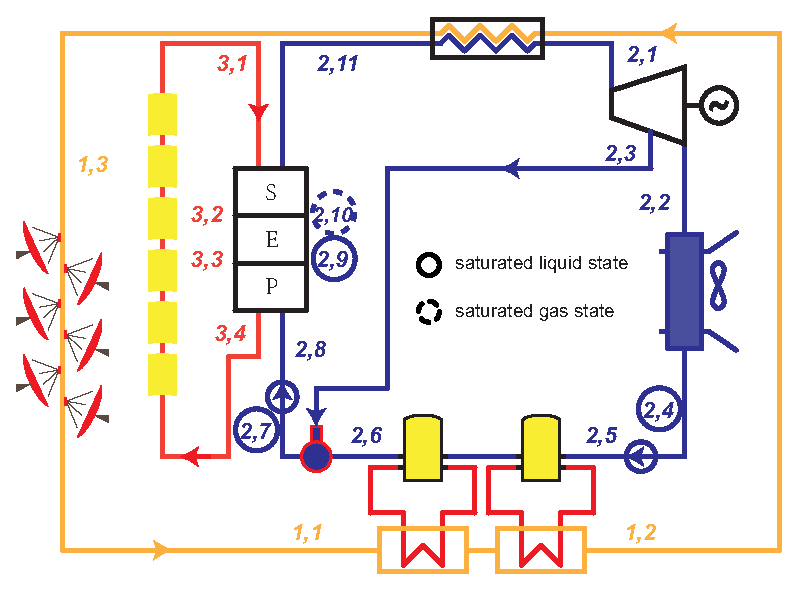
\includegraphics[width = 0.8\columnwidth]{./graphics/cascadeSystem}
	\caption{Sketch of the cascade system}
	\label{fig:System-1}
\end{center}
\end{figure}

To build the cascade system model, several simplifying assumptions are made:

\begin{itemize}
	\item Steady state at nominal load of the system is analyzed
	\item Pressure drop due to flow is negligible
	\item The leak of working fluid in the pipes is neglected
	\item Same isentropic efficiency of steam turbine with different loads and in different stages
	\item Heat loss that occurs from the tube to the atmosphere is not considered
	\item There is no heat loss to the environment for Stirling engines
	\item Simple models are used of some processes and equipments
	\item A symmetrical regenerator behaviour is assumed so that a single effectiveness can be defined as $e=\dfrac{T_R - T_L}{T_H - T_L}$\cite{Formosa2010, Juhasz2010}
\end{itemize}

%\section{System specification}
Table~\ref{tab:system-data} shows the basic design parameters of the cascade system.

\begin{table}[htbp]
	\caption{Parameters of the cascade system}
	\begin{center}
	\begin{tabular}{cc}
		\toprule
		\multicolumn{2}{c}{Nominal electric power}\\
		\midrule
		$P_{generator}$		&	6$\times10^6$ W\\
		\midrule
		\multicolumn{2}{c}{Environment}\\
		\midrule
		$I_{DNI}$			&	700 W/m$^2$\\
		$T_{amb}$			&	293 K\\
		$p_{amb}$			&	1$\times10^5$ Pa\\
		$v_{wind}$			&	4 m/s\\
		\midrule
		\multicolumn{2}{c}{Dish collector}\\
		\midrule
		$T_{dish,inlet}$	&	623K\\
		$T_{dish,outlet}$	&	1073 K\\
		$p_{dish}$			&	5$\times10^5$ Pa\\ 
		$A_{dishCollector}$	&	87.7 m$^2$\\
		\midrule
		\multicolumn{2}{c}{Trough collector}\\
		\midrule
		$\Delta{}T_{oil,water,min}$	&	15 K \\
		$T_{trough,outlet}$	&	623 K\\
		$p_{trough}$		&	2$\times10^6$ Pa\\
		$A_{troughCollector}$	&	545 m$^2$\\
		\midrule
		\multicolumn{2}{c}{Stirling engine}\\
		\midrule
		$T_{1,afterstirling}$	&	673 K\\
		$n_{se}$			&	10 s$^{-1}$\\
		$U_{stirling,1}$	&	30 W/(m$^2\cdot$K)\\
		$U_{stirling,2}$	&	150 W/(m$^2\cdot$K)\\
		$A_{stirling,1}$	&	8 m$^2$\\
		$A_{stirling,2}$	&	8 m$^2$\\
		$k_{stirling}$		&	1.4\\
		$\gamma_{stirling}	$	&	3.375\\
		$n$					&	7.73$\times{}10^{-2}$ mol\\
		$n_{stirlingEngine}$	&	100\\
		\midrule
		\multicolumn{2}{c}{Steam turbine}\\
		\midrule
		$T_s$				&	340$^\circ$C\\
		$p_s$				&	2.35$\times10^6$ Pa\\
		$p_c$				&	1.5$\times10^4$ Pa\\
		$T_{s,d}$			&	390$^\circ$C\\
		$p_{c,p}$			&	1$\times10^6$ Pa\\
		\midrule
		\multicolumn{2}{c}{Deaerator}\\
		\midrule
		$p_{deaerator}$ & 1$\times10^6$ Pa\\
		\bottomrule
	\end{tabular}
	\end{center}
	\label{tab:system-data}
\end{table}
\nomenclature{$P_{generator}$}{Power of generator, W}
\nomenclature{$I_{DNI}$}{Direct Normal Irradiance, W/m$^2$}
\nomenclature{$T_{amb}$}{Ambient temperature, K}
\nomenclature{$p_{amb}$}{Ambient pressure, Pa}
\nomenclature{$v_{wind}$}{Ambient wind speed, m/s}
\nomenclature{$T_{dish,inlet}$}{Dish inlet temperature, K}
\nomenclature{$T_{dish,outlet}$}{Dish outlet temperature}
\nomenclature{$p_{dish}$}{Air pressure in dish, Pa}
\nomenclature{$A_{dishCollector}$}{Aperture area of each dish collector, m$^2$}
\nomenclature[G]{$\Delta{}T_{oil,water,min}$}{Minimum temperature difference between oil and water in the oil-to-water heat exchanger, K}
\nomenclature{$T_{trough,outlet}$}{Trough outlet temperature}
\nomenclature{$p_{trough}$}{Air pressure in trough, Pa}
\nomenclature{$A_{troughCollector}$}{Aperture area of each trough collector, m$^2$}
\nomenclature{$T_{1,afterstirling}$}{Air temperature after heating Stirling engine}
\nomenclature{$n_{se}$}{Speed of Stirling engine, s$^{-1}$}
\nomenclature{$U_{stirling,1}$}{Overall heat transfer coefficient of Stirling engine at air side, W/(m$^2\cdot$K)}
\nomenclature{$U_{stirling,2}$}{Overall heat transfer coefficient of Stirling engine at water side, W/(m$^2\cdot$K)}
\nomenclature{$T_s$}{Main steam temperature of turbine}
\nomenclature{$p_s$}{Main steam pressure of turbine, Pa}
\nomenclature{$p_c$}{Exhaust pressure of turbine, Pa}
\nomenclature{$T_{s,d}$}{Designed mean steam temperature of turbine}
\nomenclature{$p_{cp}$}{Water pressure after condensate pump, Pa}
\nomenclature{$p_{deaerator}$}{Outlet pressure of deaerator, Pa}

\section{System model}
The system is built in several blocks. These blocks are made of circuits and efficiency calculations. Two circuits, air circuit and water circuit, are built in some specific states and in some components. Known parameters of the states, we can get the efficiency of the system and the overall efficiency of separated systems.

\subsection{Air circuit}
In air circuit, efficiency of dish collectors needs to be calculated. Fraser, in his dissertation\cite{Fraser2008}, built a performance prediction model of Stirling dish system, which has detailed description of the dish collector model. The model is also used in the software SAM\nomenclature[C]{SAM}{System Advisor Model}, which provides performance and financial models for facilitate decision in the renewable energy industry.

\noindent \begin{figure}[hp]
\begin{center}
	\includegraphics[width = 0.8\columnwidth]{graphics/dishReceiver1}
	\caption{Structure of the dish receiver}
	\label{fig:dishReceiver}
\end{center}
\end{figure}

In our cascade system, the structure of the dish receiver is as shown in Figure~\ref{fig:dishReceiver}. The dish receiver model concerns the losses includes: collector losses due to mirror reflectivity, receiver intercept losses, losses due to shading, and thermal losses. Thermal losses take the largest portion of all those losses, which are due to conduction, convection and radiation. Figure~\ref{fig:thermal-lose} shows the heat network of dish receiver, which concerns the losses:
\begin{itemize}
	\item Radiation losses reflected off of the receiver cavity surfaces and out of the receiver through the aperture. ($q_{rad,reflect}$)
	\item Conductive losses through the receiver insulating layer. ($q_{cond,tot}$)
	\item Free convection from the cavity in the absence of wind. ($q_{conv,free}$)
	\item Forced convection in the presence of wind. ($q_{conv,forced}$)
	\item Emission losses due to thermal radiation emitted from the receiver aperture. ($q_{rad,emit}$)
\end{itemize}

\noindent \begin{figure}[htbp]
\begin{center}
	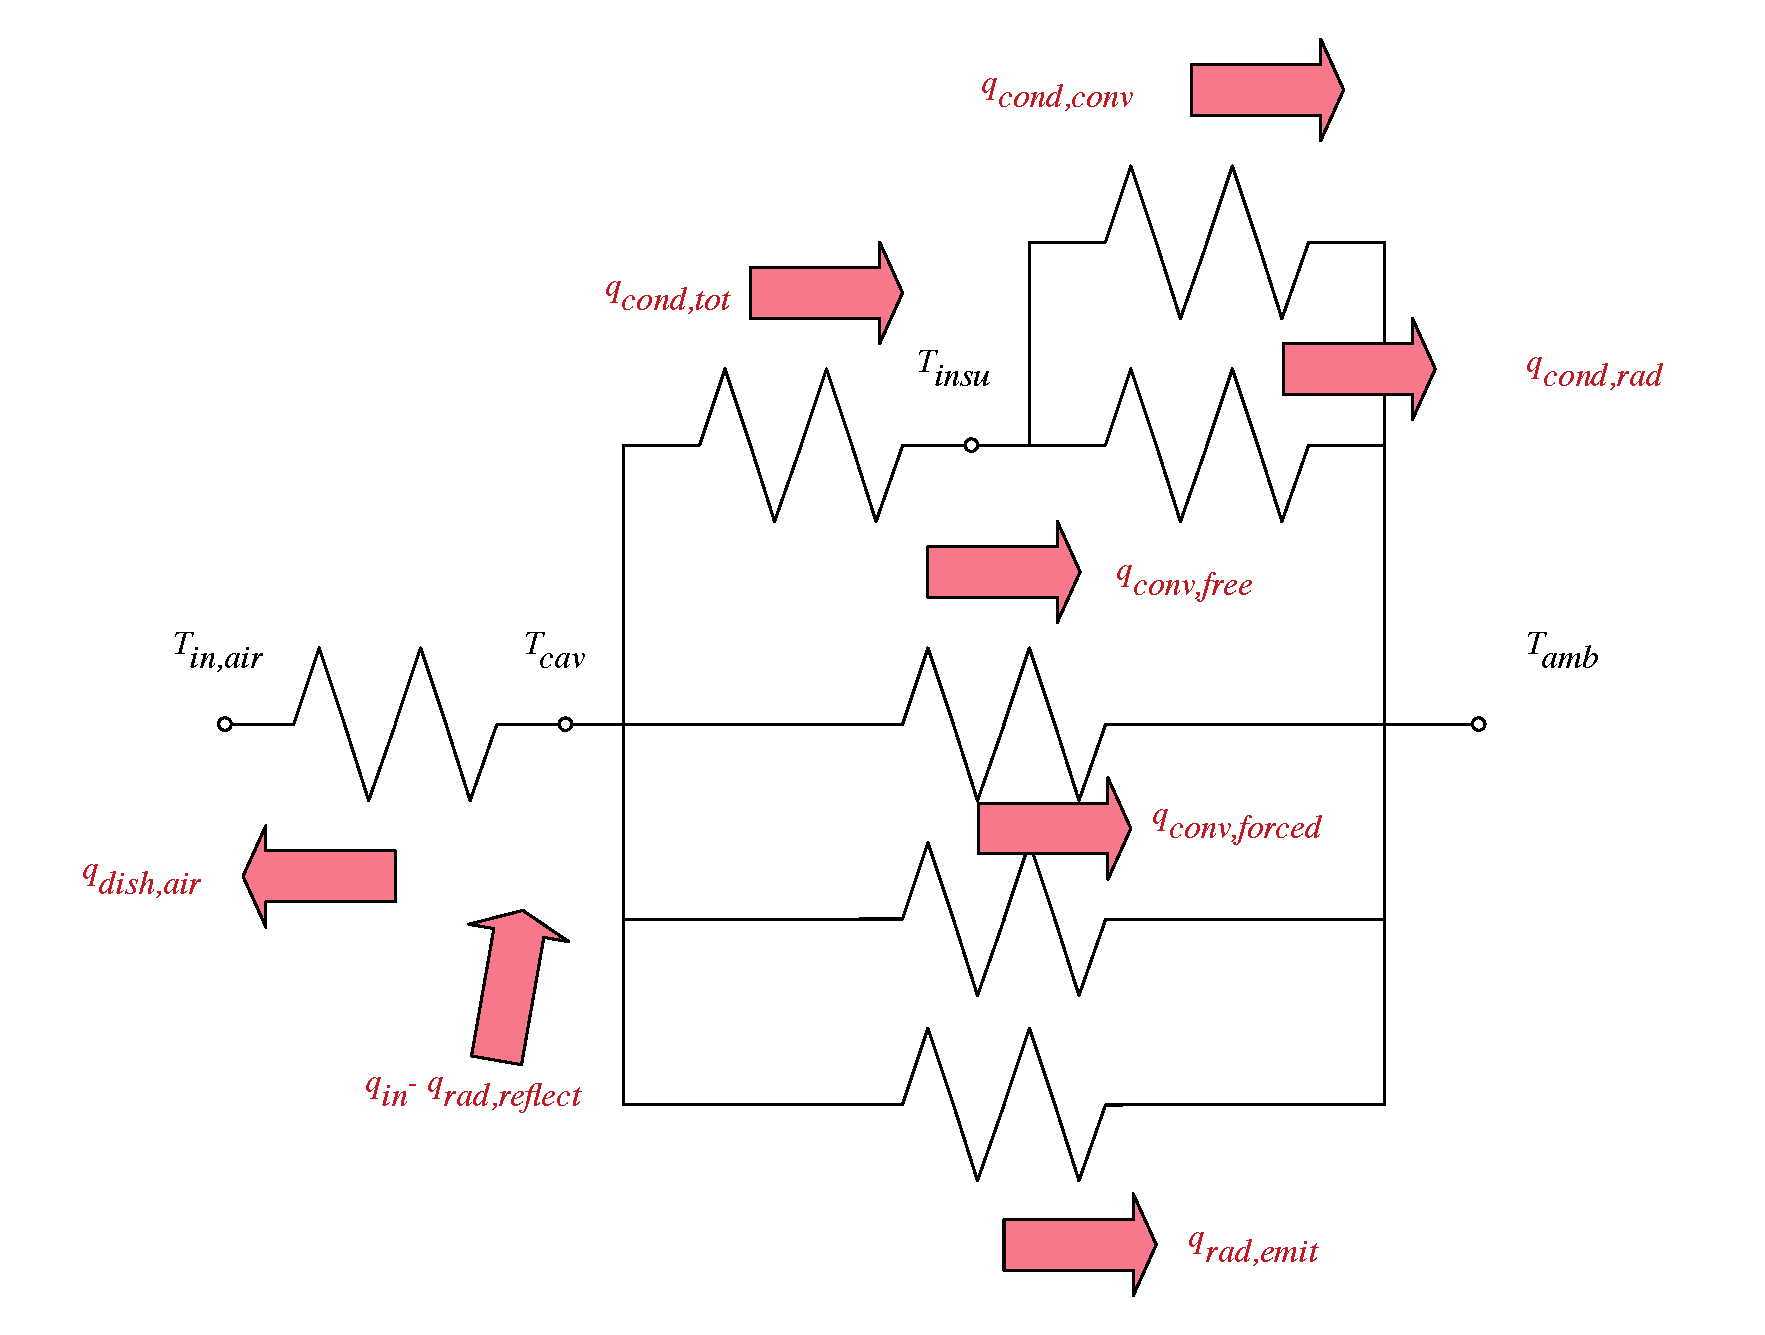
\includegraphics[width = 0.8\columnwidth]{./graphics/thermalLosses}
	\caption{Heat network of dish receiver}
	\label{fig:thermal-lose}
\end{center}
\end{figure}

\begin{equation}
\begin{aligned}
	q_{in} = q_{rad,reflect}+q_{dish,air}+q_{cond,tot}+q_{conv,tot}+
	\\q_{rad,emit}\label{eq:q_in sum}
\end{aligned}
\end{equation}
\nomenclature{$q_{in}$}{Solar energy launched into dish receiver aperture, W}
\nomenclature{$q_{rad,reflect}$}{Reflected radiation by volumetric receiver, W}
\nomenclature{$q_{dish,air}$}{Energy absorbed by air in the dish collector}
\nomenclature{$q_{cond,tot}$}{Total conduction loss}
\nomenclature{$q_{conv,tot}$}{Total convection loss}
\nomenclature{$q_{rad,emit}$}{Radiation emitted by dish receiver}

A dish collector product of SES\nomenclature[C]{SES}{Stirling Energy System} used in Fraser's paper, which is also used in this system, and its parameters are listed in Table~\ref{tab:dishReceiver} \cite{Fraser2008}. 

\begin{table}[htbp]
	\caption{Parameters of the dish receiver}
	\begin{center}
	\begin{tabular}{cc}
		\toprule
		Parameters	&	Value\\
		\midrule
		$d_{cav}$	&	0.46 m\\
		$\delta_{insu}$	&	0.075 m\\
		$l_{cav}$	&	0.23 m\\
		$d_{ap}$	&	0.184 m\\
		$\lambda_{insu}$	&	0.06 W/(m$\cdot$K)\\
		$\epsilon_{insu}$	&	0.6\\
		$\alpha_{cav}$	&	0.87\\
		$\delta_a$	&	0.005 m\\
		$d_{i,air}$	&	0.07 m\\
		$\theta_{dish}$	&	45$^\circ$\\
		$\gamma$	&	0.97\\
		$\eta_{shading}$	&	0.95\\
		$\rho$	&	0.91\\
		\bottomrule
	\end{tabular}
	\end{center}
	\label{tab:dishReceiver}
\end{table}

\nomenclature{$d_{cav}$}{Diameter of volumetric receiver cavity, m}
\nomenclature[G]{$\delta_{ins}$}{Thickness of receiver insulating layer, m}
\nomenclature{$l_{cav}$}{Depth of volumetric receiver cavity, m}
\nomenclature{$d_{ap}$}{Aperture diameter of volumetric receiver, m}
\nomenclature[G]{$\lambda_{ins}$}{Thermal conductivity of receiver insulating layer, W/(m�K)}
\nomenclature[G]{$\epsilon_{insu}$}{Emissivity of reciver insulating layer}
\nomenclature[G]{$\delta_{a}$}{Thickness of air tube in volumetric receiver, m}
\nomenclature{$d_{i,air}$}{Inner diameter of air tube, m}
\nomenclature[G]{$\theta_{dish}$}{Dish aperture angle (0$^{\circ}$ is horizental, 90$^{\circ}$ is vertically down)}
\nomenclature[G]{$\gamma$}{Intercept factor}
\nomenclature[G]{$\eta_{shading}$}{Shading factor}
\nomenclature[G]{$\rho$}{Reflectivity}
\nomenclature{$A_{stirling,1}$}{Heat transfer area of Stirling engine at air side, m$^2$}
\nomenclature{$A_{stirling,2}$}{Heat transfer area of Stirling engine at water side, m$^2$}
\nomenclature{$k_{stirling}$}{Specific heat ratio of the working gas in Stirling engine}
\nomenclature[G]{$\gamma_{stirling}$}{Compression ratio of Stirling engine}
\nomenclature{$n$}{Amount of working gas in each Stirling engine, mol}
\nomenclature{$n_{stirlingEngine}$}{Number of Stirling engines in the Stirling engine array}

$q_{in}$ can be obtained by
\begin{equation}
q_{in}=I_{DNI}\cdot A_{dishCollector}\gamma\eta_{shading}\rho\label{eq:q_in}
\end{equation}


\subsubsection{Reflected loss of dish receiver}
To determine the reflected loss of the cavity surfaces of the dish receiver, the effective absorptance of the cavity receiver $\alpha_{eff}$\nomenclature[G]{$\alpha_{eff}$}{Effective absorptance} is required to determine the fraction of energy reflected out of the receiver. The effective absorptance of a cavity receiver without a receiver aperture cover is given by Equation~(\ref{eq:alpha_eff}) where $\alpha_{cav}$ is the cavity surface absrptance, $A_a$ is the cavity aperture area, and $A_{cav}$ is the total inner surface area of the cavity \cite{Duffie2013}. Sandra National Laboratories gave an estimate value of the absorptance of the cavity surface $\alpha_{cav}$ of an existing Stirling dish receiver to be 0.87 \cite{Hogan1994}. To achieve higher effective absorptance, a smaller ratio of the two surface area should be used. But the ratio is constrained by the concentration ratio of the receiver.

\begin{equation}
	\alpha_{eff}=\dfrac{\alpha_{cav}}{\alpha_{cav}+\left(1-\alpha_{cav}\right)\left(A_{ap}/A_{cav}\right)}
	\label{eq:alpha_eff}
\end{equation}

\begin{equation*}
	q_{rad,reflect}=q_{in}(1-\alpha_{eff})
\end{equation*}

\subsubsection{Conduction loss of dish receiver}
Conduction loss of dish receiver $q_{cond,tot}$ equals to the different two parts: convection loss from the insulating layer to the atmosphere $q_{cond,conv}$ and radiation loss from the insulating layer to the atmosphere $q_{cond,rad}$. Both of the two parts are related to the temperature of insulating layer $T_{ins}$.

\subsubsection{Convection loss of dish receiver}
Ma\cite{Ma1993} conducted tests to determine the free convection losses from the receiver for six alternative setups, and the data were consistent with Stine and McDonald's free convection correlation. It is assumed that forced convection is independent of free convection in the receiver, so the total convection losses can be represented as the sum of the free and forced convection losses as shown in Figure~\ref{fig:thermal-lose}.

\begin{equation}
	q_{con,tot} = q_{con,free} + q_{con,forced}
\end{equation}

\subsection{Stirling engine array}

\subsection{Water circuit}

\subsubsection{Oil-Water heat exchangers}

\subsubsection{Steam turbine}

\subsubsection{Condensor}

\subsubsection{deaerator}

\section{Separate system model}

\section{Result and Conclusion}

\printnomenclature[2.5cm]{}
\clearpage

\bibliography{./bibliography/CascadeSystem}
\bibliographystyle{unsrt}

\end{document}